\chapter{基于Spring MVC框架的WEB应用开发}
\label{cha:web}
本章首先介绍WEB应用开发的主要程序语言,然后对Spring MVC框架进行了详细的介绍。同时,对各种技术的应用反问做了初步的探讨,为后文系统性能优化工作做好理论工具上的准备。
\section{应用开发语言}
目前WEB应用开发主要分为前端开发和后端开发,其中前端开发以HTML和JavaScript结合为主,后端开发语言则比较多,主流的有C语言、PHP语言、JAVA语言以及Python语言等语言,不同语言之间的作用和特点都不同,但在提高系统稳定性和系统兼容性方面JAVA语言更有优势~\cite{suzumura2008performance}。
\subsection{JAVA语言}
\subsubsection{JAVA语言产生及发展}
JAVA语言是在20世纪90年代产生的,任职于太阳微系统的詹姆斯·高斯林等人于1990年代初开发Java语言的雏形,最初被命名为Oak,目标设置在家用电器等小型系统的程序语言,应用在电视机、电话、闹钟、烤面包机等家用电器的控制和通信~\cite{byous1998java}。由于这些智能化家电的市场需求没有预期的高,Sun公司放弃了该项计划。随着1990年代互联网的发展,Sun公司看见Oak在互联网上应用的前景,于是改造了Oak,于1995年5月以Java的名称正式发布。Java伴随着互联网的迅猛发展而发展,逐渐成为重要的网络编程语言~\cite{java维基百科}。

在所有的编程语言中,应用最广泛的莫过于JAVA语言,该语言在面向对象的程序开发中一直有着突出的表现。因此在最近10几年间,JAVA语言一直保持在编程语言排行的前两名,参见图~\ref{fig:tiobe}。
\begin{figure}[H] % use float package if you want it here
  \centering
  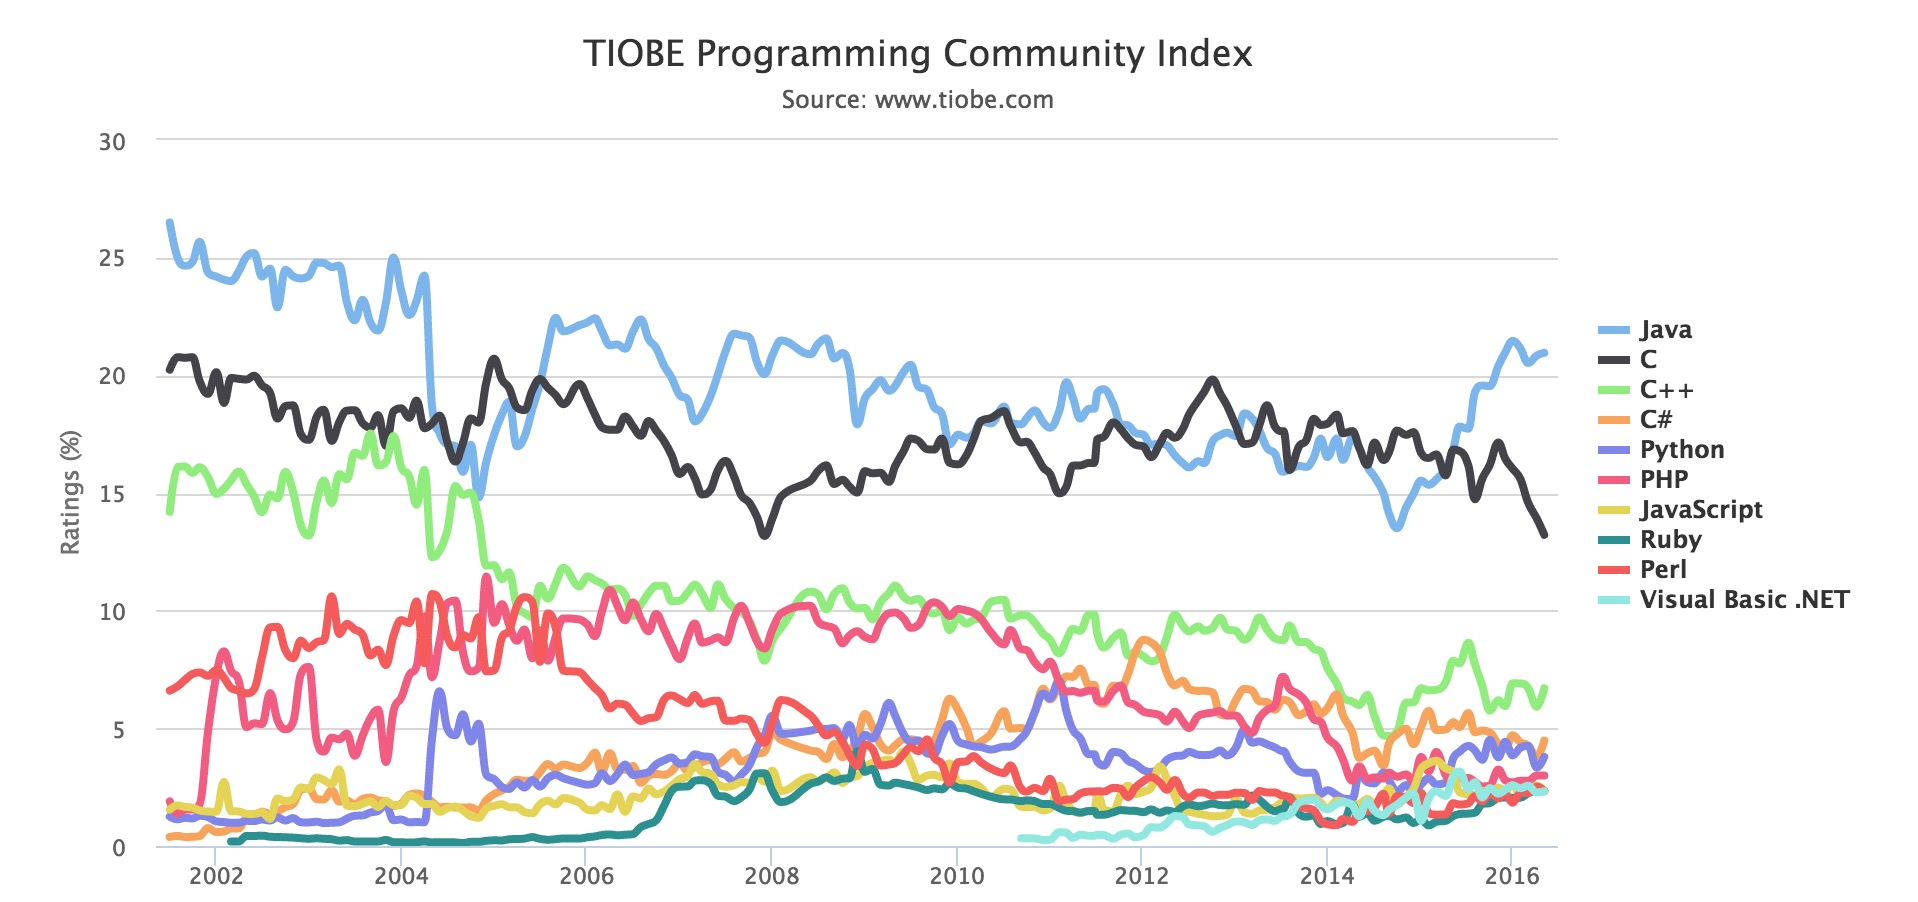
\includegraphics[width=6in]{chap02/1-TIOBE}
  \caption{编程语言近年排行}
  \label{fig:tiobe}
\end{figure}
\subsubsection{JAVA语言特点}
因特网的普及推动了JAVA语言的发展,同时JAVA语言在网页制作上的应用也丰富了因特网的内容。两者可谓是相辅相成、相互促进。JAVA语言的特点如表\ref{tab:java-1}。
\begin{table}[htb]
  \centering
  \begin{minipage}[t]{0.8\linewidth} % 如果想在表格中使用脚注,minipage是个不错的办法
  \caption[模板文件]{模板文件。如果表格的标题很长,那么在表格索引中就会很不美
    观,所以要像 chapter 那样在前面用中括号写一个简短的标题。这个标题会出现在索
    引中。}
  \label{tab:java-1}
    \begin{tabularx}{\linewidth}{lX}
      \toprule[1.5pt]
      {\heiti 特点} & {\heiti 描述} \\\midrule[1pt]
      可移植性 & 能移植于不同的使用平台,扩大了系统的使用范围 \\
      面向对象 & 集成了C++的优点,并且在面向对象方面有新的扩展 \\
      多线程 & 可以让多个不同处理器同时进行工作,是数据库系统开发的最佳选择 \\
      分布式 & 在处理TCP等协议的同时也支持网络编程\\
      \bottomrule[1.5pt]
    \end{tabularx}
  \end{minipage}
\end{table}
\section{Spring MVC开发框架}
Spring MVC 是一种基于Web开发的系统架构,目前主流的系统框架还有Struts,但是Spring MVC架构引起优势依然处于不可替代的位置。在Spring MVC架构中,系统的终极目标被解聚、分块,并在不同的模块中表达出来,如此系统的耦合度得到大幅降低。同时,该框架的整体运行也是在模块驱动的基础之上的,用户首先发出请求,然后系统予以相应,即常规的请求-相应模型。
\subsection{Spring MVC 架构的特点}
Spring MVC 架构不同于传统的体系架构,在其发展的过程中吸收其他系统的特点,如支持Userful风格,灵活的本地化等。这些特征保证了Spring MVC框架在发展过程中,更加受到开发者的青睐。同时,吸收了前人的经验以后,Spring MVC框架也具备专属的特点,比如用Spring MVC框架设计的WEB系统其耦合度较低,系统总体表现出简洁明了的风格,这样用户就能更快捷的掌握数据库系统的操作~\cite{林薇2015基于}。

Spring MVC框架是在Spring框架的基础上发展起来的,因此Spring MVC框架集成了Spring 框架的所有功能,而且两者在相互继承方面表现出很好的融合性。这一特点给系统开发带来了很多方便。除此之外,Spring MVC模型在图形兼容性和数据验证的灵活性上都有先天的优势。正式因为这些特点,使Spring MVC模型在实际应用中发挥出巨大的优势,同时也在程序员中受到青睐。本文的WEB应用就是建立在该框架之上的。
\subsection{Spring MVC 框架处理流程}
Spring MVC架构是一个基因用户请求的系统架构,其过程也要求有Web驱动的参加。具体过程现有用户发送请求到前端控制器,这时候前端控制器将请求委托给处理器;于是处理器就开始处理请求,即调用业务对象进行分析,分析完毕后将模型数据返回给处理器;然后处理器再将处理结果通过模型和视图返回给前端控制器;此时前端控制器显示的数据用户还无法处理,还需要进行视图渲染,最终在前端控制器显示出来,即用户发送的请求产生了响应。整个过程参见图~\ref{fig:mvc},此图反映了用户请求-响应的过程。
\begin{figure}[H] % use float package if you want it here
  \centering
  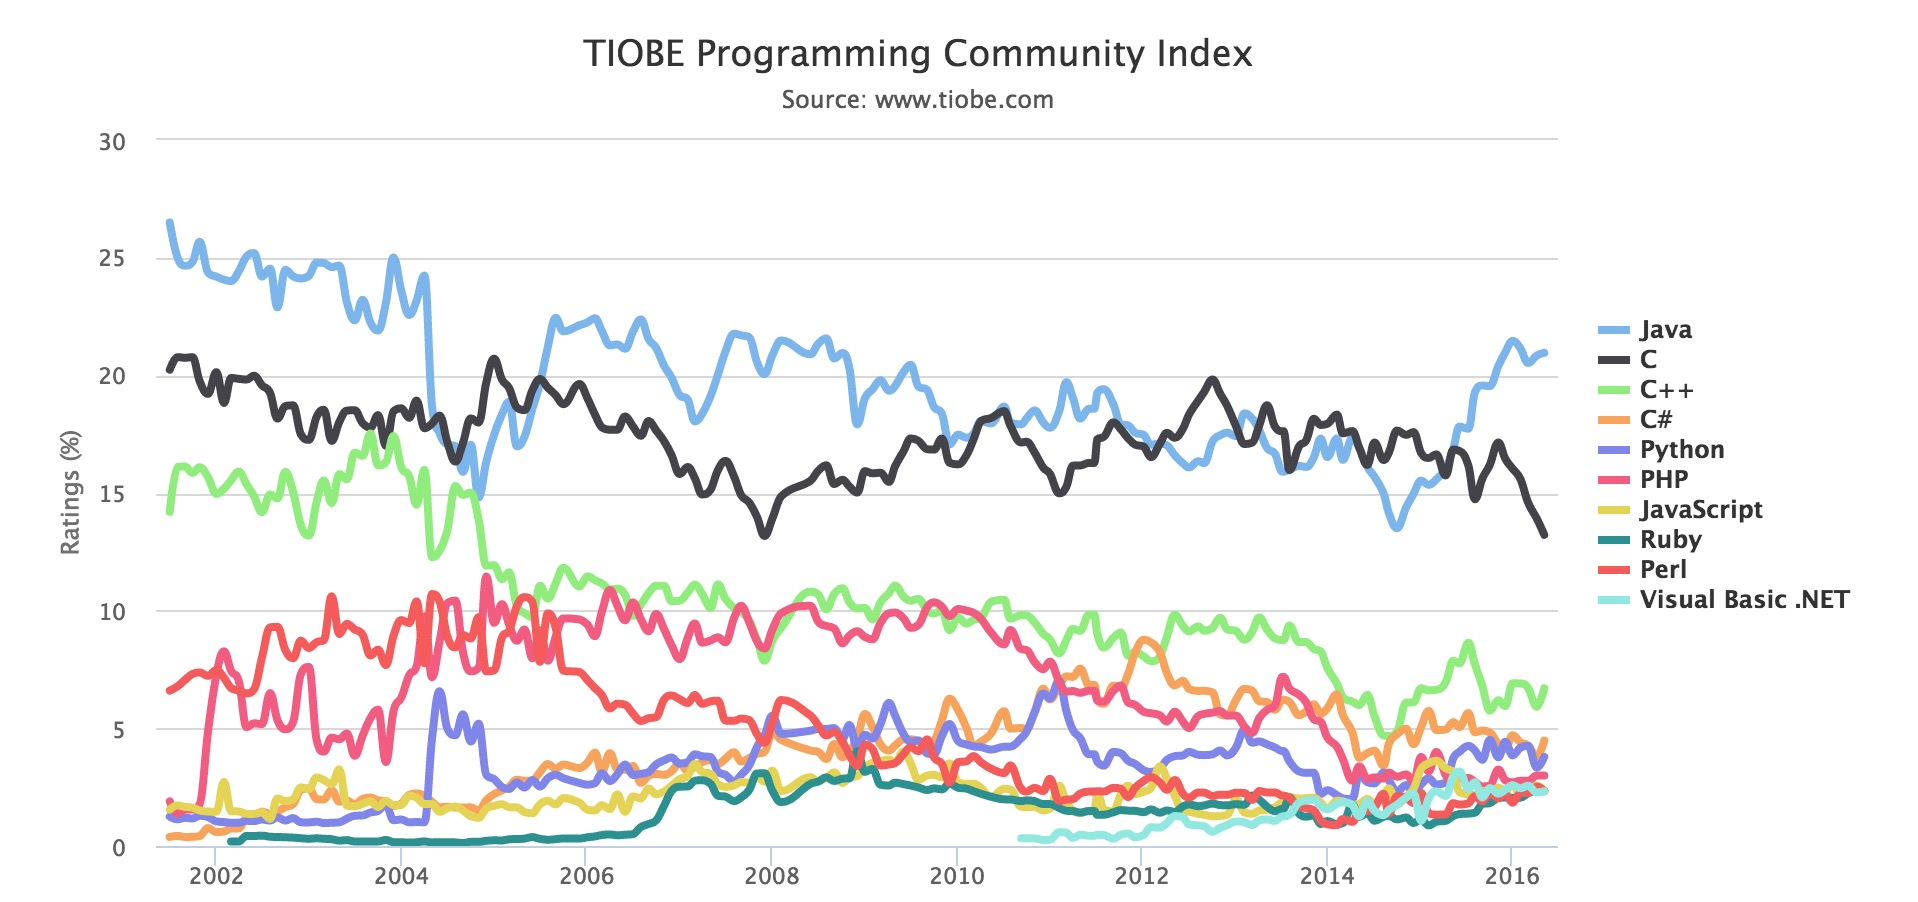
\includegraphics[width=6in]{chap02/1-TIOBE}
  \caption{编程语言近年排行}
  \label{fig:mvc}
\end{figure}
\subsubsection{体系的三层架构}
MVC(Model View Controller), 即视图、模型和控制器三个英文单词的首字母缩写,按照应用的流程本系统可以在Spring MVC架构下分为三层,具体的架构为显示层、控制层和数据访问层。

\begin{enumerate}
\item 显示层。主要有Spring和JSP经过页面REQUEST请求,Spring的URL Mapping对应到响应的控制器,通过对页面发送的请求,Spring自动的去寻找响应的控制类,并将结构展示在页面上。

\item 控制层。也就是业务层,是系统中最重要的一层,这层主要是接受URL发送过来的业务请求,然后去访问Service层,把需要的数据装入缓存中,任何通知Action进行跳转。

\item 数据访问层。 这层最重要的作用是对数据库中数据以及XML文件中的数据进行访问及操作,并把操作的结果反馈到业务逻辑层,将相应的结果交由下一层去处理。
\end{enumerate}
这个三层架构的体系的应用很好的解决了系统资源的分配问题,而且将系统的耦合度降到了可以接受的最低水平。同时,关于异步处理问题上,本系统使用了FDP框架,FDP框架是对AJAX的一种轻量级的封装,它的目标是使AJAX和XML Http Request更简单。通过FDP框架,我们只需要在相应的配置对应的JAVA方法以及相对于的实体类,我们很容易的就可以实现许多异步操作,使一些操作不用刷新页面即可达到相应的效果。可以认为FDP框架是对MVC三层框架的一种拓展,其本质还是在MVC框架内的。由此可见,笔者在系统体系的选择上更倾向于架构简单、可移植性好的系统框架模型。
\section{应用开发工具}
在开发基于Spring MVC的WEB应用过程中,需要用到的基础编程语言是JAVA,系统的架构采用的MVC三层架构。这些都属于手段,但是想要达到最终目的则需要用到一些基础的软件工具,这些工具的使用将加快工作效率。
\subsection{IntelliJ IDEA}
IntelliJ IDEA 是一款Java集中开发环境工具软件,由捷克软件公司JetBrains在2001年1月时推出最初版~\cite{jemerov2008implementing}。该软件被认为是当前Java开发效率最快的IDE工具。它集成了开发过程中实用的众多功能,几乎可以不用鼠标可以方便的完成你要做的任何事情,最大程度的加快开发的速度。简单而又功能强大。与其他的一些繁冗而复杂的IDE工具有鲜明的对比~\cite{IDEA维基百科}。
\subsection{Maven}
Apache Maven是由Apache软件基金会所提供德一个项目管理及自动构建工具~\cite{smart2005introduction}。它基于项目对象模型概念、能够实现一个Java项目的构建和依赖管理。本论文所涉及的WEB应用就是使用Maven来构建Java Web项目。
\subsection{Tomcat}
WEB应用的Web服务器采用的是有Apache软件基金会(Apache Software Foundation)下属的Jakarta项目开发的一个Servlet容器,由于其本身也包含一个HTTP服务器,因此也常常被用作一个单独的Web服务器~\cite{brittain2007tomcat}。Tomcat7支持最新的Servlet 3.0规范,而且技术先进、稳定性强一级免费的特点,深受Java爱好者的喜爱并得到了部分软件开发商的认可,成为目前比较流行的Web应用服务器。
\subsection{MySQL}
MySQl是个小型关系型数据库管理系统,之所以使用MySQL是因为MySQL是一款免费的数据库管理系统,而且其建议的操作以及其兼容性都是其优点~\cite{greenspan2001mysql}。MySQL的特点主要有:
\begin{itemize}
\item 为多种編程语言提供了API。这些編程语言包括C、C++、C$\sharp$、Java、Perl、PHP、Python、Ruby等。
\item 支持多线程,充分利用CPU资源,支持多用户。
\item 提供TCP/IP、ODBC和JDBC等多种数据库连接途径。
\item 提供用于管理、检查、優化数据库操作的管理工具。
\item 可以处理拥有上千万条记录的大型数据库。
\end{itemize}
\subsection{Couchbase}
在互联网时代,我们面对的是更多的客户端,更低的请求延迟,这就需要对数据做大量的Cache以提高读写速度~\cite{brown2012getting}。目前主流的Cache系统memcached和redis虽然有很熟的解决方案,但是也都有其局限性~\cite{kovacs2013cassandra}:
\begin{itemize}
\item Cluster 支持不够。在扩容、负载均衡、高可用等方面存在明显不足。
\item 持久化支持不好,出现问题后恢复的代价大。memcached 完全不支持持久化,redis 的持久化会造成系统间歇性的负载很高。
\end{itemize}
Couchbase是一个NoSQL数据库,它是世界各国的开发者在2011年推出的,由于它有良好的cluster支持、异步持久化的支持得到了众多开发者的青睐,他的特点主要有:
\begin{itemize}
\item Couchbase 的对等网设计,smart client 直接获取整的集群的信息,在客户端实现负载均衡,整个集群没有单点失效,并且完全支持平行扩展。
\item vBucket 的引入,完全实现了 auto sharding,可以方便灵活的把数据的子集在不同节点上移动,以实现集群动态管理。
\item Couchbase 有一个非常专业的 web 管理界面,并且支持通过 RESTful API 管理,这也是 memcached, redis 不能企及的。
\end{itemize}
\section{应用开发流程}
WEB应用在开发的时候设计为前后端分离,通过FDP框架实现前端到后端的请求,所以本论文测试WEB应用的开发主要分为三个方面。
\subsection{前端开发}
应用的前端相当于MVC架构中的视图层,在前端开发中,通过Html和JavaScript来设计实现应用的页面展示,通过FDP的Ajax请求将前端的用户请求转发到应用的后端。
\subsection{后端开发}
应用的后端主要分成了Controller、Service、Pst三层,其中Controller层负责处理用户的请求然后将业务转发给Service层,Service层负责实现用户的请求,通过设计不同的业务逻辑将用户需要的数据返回,涉及到数据的读取则通过Pst层,Pst层主要负责对数据库的增删改查,将结果返回到Service层。
\subsection{数据库搭建}
应用的数据主要分为基础数据也业务数据,其中基础数据主要包括页面的功能板块、系统的定时任务、数据的权限设置、页面的功能逻辑等数据,业务数据主要包括用户的信息、用户操作记录、用户的商店、商品、销售信息等。
\section{基于Jenkins的持续集成方案开发}
在每一次WEB应用的开发、上线过程中,不可避免的要将本地环境打包上传到生产环境或者是测试环境进行解压,每一次人工的干预无疑增加了时间成本,通过Jenkis设计实现应用的持续集成,这在很大程度上能够帮助开发着实现快速的应用部署和错误重现。

Jenkins是一个用Java编写的开源的持续集成工具,它提供了软件开发的持续集成服务,运行在Servlet容器中,它可以执行基于Apache Ant和Apache Maven的项目,以及任意的Shell脚本和Windows批处理命令。
\section{本章总结}